\documentclass[compress]{beamer}

%--------------------------------------------------------------------------
% Common packages
%--------------------------------------------------------------------------
\usepackage[english]{babel}
\usepackage{pgfpages} % required for notes on second screen
\usepackage{graphicx}
\usepackage{subfigure}
\usepackage{multicol}
\usepackage[normalem]{ulem}

\usepackage{tabularx,ragged2e}
\usepackage{booktabs}
\usepackage{marvosym}

%--------------------------------------------------------------------------
% Load theme
%--------------------------------------------------------------------------
\usetheme{hri}

\usepackage{tikz}
\usetikzlibrary{shapes,fpu,fit,calc,mindmap,backgrounds,positioning,svg.path}

\tikzset{
    invisible/.style={opacity=0},
  visible on/.style={alt={#1{}{invisible}}},
  alt/.code args={<#1>#2#3}{%
      \alt<#1>{\pgfkeysalso{#2}}{\pgfkeysalso{#3}} % \pgfkeysalso doesn't change the path
  },
}

\graphicspath{{figs/}}


%--------------------------------------------------------------------------
% General presentation settings
%--------------------------------------------------------------------------
\title{Cognition and Social Robots}
\subtitle{Investigating the emergence of artifical social cognition}
\date{INRIA Flowers -- {\bf 10th January 2017}}
\author{Séverin Lemaignan}
\institute{Centre for Robotics and Neural Systems\\{\bf
Plymouth University}}

%--------------------------------------------------------------------------
% Notes settings
%--------------------------------------------------------------------------
%\setbeameroption{show notes on second screen}
%\setbeameroption{hide notes}

\begin{document}

\licenseframe{https://github.com/severin-lemaignan/presentation-cognitive-robotics}
\maketitle

%%%%%%%%%%%%%%%%%%%%%%%%%%%%%%%%%%%%%%%%%%%%%%%%%%%%%%%%%%%%%%%%%%%%%%%%%%%%%%%
%%%%%%%%%%%%%%%%%%%%%%%%%%%%%%%%%%%%%%%%%%%%%%%%%%%%%%%%%%%%%%%%%%%%%%%%%%%%%%%
%%%%%%%%%%%%%%%%%%%%%%%%%%%%%%%%%%%%%%%%%%%%%%%%%%%%%%%%%%%%%%%%%%%%%%%%%%%%%%%
\section{Framing the research}
\subsection{Starting point}
 \begin{frame}{Our starting point}

        {\bf Symbolic artificial social cognition}:
        works rather well as long as:
        \begin{itemize}
            \item we know what we want to do (in terms of task domain,
                \& declarative knowledge)
            \item interaction mostly relying on symbolic \emph{perceptual inputs}
                (including visual perspective taking) rather abstract or less
                explicit representations
        \end{itemize}
        \pause

        Good for any practical HRI purposes? {\bf mostly}!
        \pause

        Intuitively, social modeling goes beyond computing what the human
        perceives or does not perceive $\rightarrow$ Flavell's \emph{cognitive
        connections} vs \emph{mental representations}.

        Symbolic cognition {\bf does not explain much about how social cognition actually
        work}. We need a {\bf principled approach} to social cognition for robots

 \end{frame}

\subsection{Goals}
\begin{frame}{A long-term direction}

    Adapting and unifying the large and disparate set of theories on social
    cognition to {\bf build a theory of social cognition for
    robots}

    \pause
    ...or rather, {\bf a computational model of social cognition for robots}

    \pause

    ...or rather, an {\bf embodied} computational model of social cognition?

    \footnotesize (we'll come back to this in a moment)

\end{frame}

\begin{frame}{One question}

    \Large
    \centering

    Can sociality emerge from interaction?

    \pause
    \normalsize
    \vspace{2em}

    Both ``emerge'' as \emph{arise from} and ``emerge`` as in \emph{emergent paradigm of
    cognition}!

    \pause

    ``Social cognition arising in interaction''? certainly looks like a situated \&
    embodied view on cognition

\end{frame}

\subsection{A model of social cognition}
{
    \paper{cited in Lewandowsky and Farrell, {\bf Computational Modeling In
    Cognition}, 2011}
\begin{frame}{A model?}

    Models attempt to \emph{explain}: 
    \begin{quote}
        ``identifying the causes for an event or phenomenon of interest''
    \end{quote}
    \begin{quote}
        ``unifying disparate phenomena''
    \end{quote}

        A model's value is gained from
    \begin{quote}
        ``predicting facts that, absent the theory, would be antecedently
        improbable''
    \end{quote}

    \pause

    ...we will come back to the predictive power of a model of artifical social
    cognition.

\end{frame}
}

{
    \paper{Baxter, Lemaignan, Trafton {\bf Workshop on Cognitive Architectures for Social
    Human-Robot Interaction} HRI 2016}
\begin{frame}{Cognitive Architecture as a methodology}

    \begin{center}
        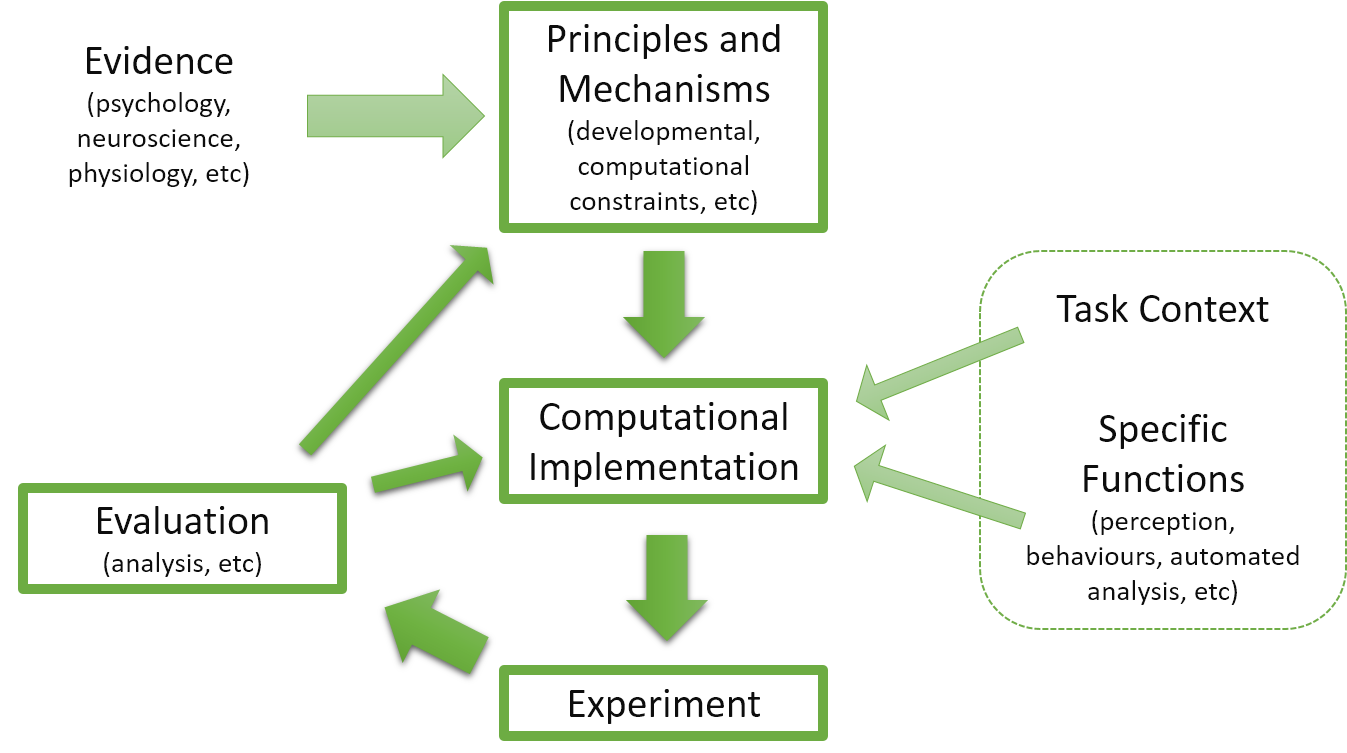
\includegraphics[width=\linewidth]{cogarch-methodology}
    \end{center}

        \badge{europe_plym}
\end{frame}
}

\section{Sketching a model}
\subsection{Postulates}
\begin{frame}{A model of artificial social cognition}

    I postulate {\bf two stages}:

    \begin{enumerate}
        \item building models of others' minds
        \item exploiting these models to socially act:
            \begin{itemize}
                \item prediction, reading others' intentions
                \item adapting own behaviour, alignment
                \item establish join goals
                \item ultimately, performing joint actions
            \end{itemize}
    \end{enumerate}

    \vspace{2em}
    $\rightarrow$ Social analogs of \emph{perception} \& \emph{action}

\end{frame}

{
    \paper{see discussion in Vernon, {\bf Artificial Cognitive Systems: A Primer} 2014}
\begin{frame}{Cognitivist vs Emergent paradigms}

    ``building'', ``exploiting'', ``reading'', ``establishing''... my terminolgy
    denotes a cognitivist approach (`I, the designer of the system, explicitly implement
    these capabilities')

    \pause
    
    Reformulation in the emergent paradigm:

    \begin{enumerate}
        \item developing internal states \emph{connoting} others' minds
        \item perturbing (influencing) actions synthesis with these states
    \end{enumerate}

    \pause

    Hybrid approaches are possible -- mapping to ``phenomenal experience'' vs
    ``access counciousness''.
\end{frame}
}

\subsection{Graziano's attention theory}
{
    \paper{Graziano {\bf Consciousness and the Social Brain} -- 2013}
\begin{frame}{Modeling others' mind?}
    \large
    In cognitive neurosciences: Graziano's \emph{Attention Schemata Theory}

    \begin{columns}

        \begin{column}{0.5\linewidth}

            \begin{center}
                \includegraphics<1>[width=1.3\columnwidth]{playing_together}
                \includegraphics<2>[width=1.3\columnwidth]{playing_together_gaze}
                \includegraphics<3>[width=1.3\columnwidth]{playing_together_awareness}
                \includegraphics<4>[width=1.3\columnwidth]{playing_together_mutual_awareness}
            \end{center}

        \end{column}

        \begin{column}{0.5\linewidth}

            \only<2>{
                \vspace*{1.5cm}
                Attention is more about {\bf representation} than visual perspective

                \vspace{0.7cm}
                ``Awareness is a construct that represents the attentional state
                of a brain''

            }
            \only<3>{
                \vspace*{1.5cm}
                Graziano's postulate that modelling other's state of awareness
                is {\bf mediated by one's own attentional system}, through joint
                attention
            }
            \only<4>{
                \vspace*{1.5cm}
                    It follows that {\bf joint attention is the process that gives
                    rise to social awareness}
            }

        \end{column}

    \end{columns}

\end{frame}
}

\subsection{Applied to robotics}
\begin{frame}{Sketching a path forward: mentalizing}

    {\bf Hypothesis 1}: Graziano is right: mental representations are snapshots of
    \emph{awareness}, \emph{awareness} being itself a label for the
    \emph{memory-mediated process of attention}.

    \pause

    {\bf Hypothesis 2}: this can be extended to social cognition. \textbf{Modeling one
    other mental representations equates to taking snapshots of their current
    state of awareness}.

    As we do not have direct access to others' process of attention, it has to
    be mediated. Following Graziano, we hypotesise that \textbf{modelling other's
    state of awareness is mediated by one's own attentional system, through
    joint attention mechanisms}.


\end{frame}

{

    \paper{Graziano's Attention Schemata Theory; Desimone and Ducan {\bf Biased Competition
Model of Attention} 1995; Block 1996}

\begin{frame}{In more details}
\footnotesize
    \begin{enumerate} \item<+-> {\bf mental representations} are {\bf snapshots
                of what we are aware of}

        \item<+-> {\bf awareness} is the label we conveniently put on the {\bf
            process of attention}

        \item<+-> attention at time t is the label we put on the set of the {\bf
            activated units} in a (biased) {\bf associative memory network}

        \item<+-> modelling {\bf others’ mental representations} is taking
            snapshots of their own current state of awareness

        \item<+-> modelling other’s state of awareness, \ie their current
            attentional process, is {\bf mediated by one’s own attentional
            system}, typically through {\bf joint attention} mechanisms

        \item<+-> Points 1 to 5 essentially refer to a \emph{phenomenal}
            awareness (a \emph{raw} inner experience). \emph{Phenomenal}
            awareness can be turned into \emph{access consciousness} (the
            abstract, cognitive ability to reflect on the inner experience)

        \item<+-> In robots, \emph{access consciousness} can be mapped to {\bf
            symbolic representations}

    \end{enumerate}


\end{frame}
}

\begin{frame}{An hybrid model of cognition}

    \begin{itemize}
        \item \emph{phenomenal experience} modelled in a connectionist
            (sub-symbolic) fashion (associative
    memory network)
\item \emph{access conciousness} in a cognitivist (symbolic) fashion (typically,
    an ontology or epistemic logics)

    \end{itemize}

    $\Rightarrow$ bottom-up

    \pause

    The \emph{Biased Competition Model of Attention} supports bottom-up as well
    as {\bf top-down biasing mechanisms}: 
    
    \begin{itemize}
        \item \emph{bottom-up}: if a unit is
            activated longer/stronger, it biases the resulting attention to this
            unit.
        \item \emph{top-down}: abstract cognitive process can influence the memory network
            to bias the attention process. Practically less clear, but also potentially very interesting
            as it {\bf closes the loop between the emergent and cognitivist
            paradigms}

    \end{itemize}

\end{frame}

\begin{frame}{Many gaps calling for investigation!}

\footnotesize
    \begin{itemize}

        \item<+-> mental representations as instantaneous 'snapshots' is a {\bf strong
            assumption} (and what about representation of lasting situations?)

        \item<+-> if attention is the set of activated units in a memory network,
            {\bf what are the units?} physical entities? social events? situations?
            what is the right level of abstraction: from raw perceptual inputs to
            high-level units like objects, joint gazing, etc.


        \item<+-> {\bf the mapping} between 'phenomenal consciousness' and
            'access consciousness' and, respectively, sub-symbolic and symbolic
            computational structures {\bf might be naive}. This need to be
            better evidenced, if only because the frontier between phenomenal
            and access consciousness is all but clear (as pointed by Graziano).

        \item<+-> what is the {\bf social motivation} for the robot to carry
            over this modeling? What social drives?

        \item<+-> at epistemic level, if access to other's mental
            representations is \emph{mediated} by one's own attentional system,
            these mental representations are subjective. {\bf Can we equate humans'
            and robots' subjectivities?}

    \end{itemize}

\end{frame}


\begin{frame}{Sketching a path forward: social behaviours}

    {\bf Hypothesis 3}: together, representations of one's and others' minds are
    \emph{necessary} and \emph{sufficient} for social behaviours to emerge

    {\bf Hypothesis 3'}: representations of one's and others' minds, along with
    a situation (physical and temporal environment), are \emph{necessary} and
    \emph{sufficient} conditions for social behaviours to emerge

    \pause

    How?


\end{frame}

\subsection{Model's predictions}
\begin{frame}{What could the model predict?}

    \begin{itemize}

        \item {\bf behavioural alignment}: each time we play together, our
            interaction flow improves, becomes more natural

        \item ability to pass {\bf false-belief tasks}, including
            non-perceptual, non-physical, abstract ones,

        \item {\bf recursive awareness}: \emph{being aware of being aware} -- typically
            evidenced by being able to describe/verbalize its own state of
            awareness 

        \item {\bf 'natural' (\ie emergent) turn-taking}: I 'just' know when it is my
            turn to act

        \item {\bf 'natural' protodeclarative pointing}: I 'just' know when I really
            need to draw your attention on something

        \item {\bf Emergence of Parten's hierarchy?}

    \end{itemize}

\end{frame}

\videoframe[0.56]{figs/next/maud-zoe-pilot-edit.mkv}

{
    \paper{Parten, {\bf Social participation among preschool children} Journal
    of Abnormal and Social Psychology 1932}
\begin{frame}{In Developmental psychology: stages of play}

    Parten's {\bf stages of play}:

    \begin{enumerate}
        \item<1-> {\bf Solitary (independent) play}: Playing separately from
            others, with no reference to what others are doing.
        \item<2-> {\bf Onlooker play}: Watching others play. May engage in
            conversation but not engaged in doing. True focus on the children at
            play.
        \item<3-> {\bf Parallel play} (adjacent play, social coaction): Playing
            with similar objects, clearly beside others but not with them (near
            but not with others.)
        \item<4-> {\bf Associative play}:  Playing with others without
            organization of play activity. Initiating or responding to
            interaction with peers. 
        \item<5-> {\bf Cooperative play}: Coordinating one’s behavior with that
            of a peer. Everyone has a role, with the emergence of a sense of
            belonging to a group. Beginning of "team work."
    \end{enumerate}

\end{frame}
}

%%%%%%%%%%%%%%%%%%%%%%%%%%%%%%%%%%%%%%%%%%%%%%%%%%%%%%%%%%%%%%%%%
%%%%%%%%%%%%%%%%%%%%%%%%%%%%%%%%%%%%%%%%%%%%%%%%%%%%%%%%%%%%%%%%%
%%%%%%%%%%%%%%%%%%%%%%%%%%%%%%%%%%%%%%%%%%%%%%%%%%%%%%%%%%%%%%%%%
\section{Experimental investigation}

\subsection{Experimental framework}
\begin{frame}{An experimental framework for investigation}

    \begin{itemize}
        \item<1-> Typical socio-cognitive tasks are either toy scenarios (\ie do not mirror
            real-world siutation) or simple, constraint tasks that do not
            reflect the complexity \& dynamics of real-world interactions
        \item<2-> $\Rightarrow$ {\bf free play}: richer set of cognitive and
            social dynamics; importance of motivation/drive; forces us to deal
            with uncertain and unexpected situations
        \item<3-> Challenge to isolate behaviours, analyses them (and if we are
            to avoid Wizard-Of-Oz, implementation challenge!)
    \end{itemize}
\end{frame}


\begin{frame}{An experimental framework}

    \begin{itemize}
        \item The ``Zoo design'' play situation
        \item {\bf Free play} with the following constraints:
            \begin{itemize}
                \item initial prompt (``Let's build a zoo!'')
                \item limited set of tokens (cubes, Lego animals)
                \item spatially limited playground
            \end{itemize}
        \item<2-> to make it technically tractable with robots, the physical
            playground is {\bf replaced by a large touchscreen} (sandtray): entirely
            skips the difficult problem of perception and manipulation in a
            dense \& cluttered scene
        \item<2-> the touchscreen strictly
            replace the perception of objects on the playground (exports
            ROS TF frames of each object) and their manipulation (receives
            virtual 'touches' from the robot)
        \item<2-> importantly, perception of the partner and of the global scene
            geometry is genuine
    \end{itemize}
\end{frame}

\imageframe[color=black]{next/zoo-activity2}
\imageframe[color=black]{next/zoo-activity}
\videoframe[0.56]{figs/next/zoo-builder-proto-smaller.mkv}


{
\paper{Lemaignan et al., {\bf From Real-time Attention Assessment to
“With-me-ness” in Human-Robot Interaction} HRI 2016}
\begin{frame}{An experimental framework}

    Open-ended task: more an {\bf experimental framework} than a task.

    \begin{itemize}
        \item free play, yet sufficiently well-defined to be reproducible
        \item focus on abstract socio-cognitive facets (perception is simplified;
            manipulation is mostly avoided)
    \end{itemize}
    
    Besides, well suited for interaction analysis, with tools like:
    \begin{itemize}
        \item behavioural alignment between partners: for instance, using
            Słowinski's \emph{Individual Motor Signature}
        \item Ballard's (and Anderson's extension) coding of children's free-play interactions
        \item \emph{With-me-ness} as a metric of co-engagment
    \end{itemize}
\end{frame}
}

\section{La route est encore longue}
\subsection{What's next?}
\begin{frame}{Open questions}

    The most obvious one: {\bf what cognitive architecture?}

    $\rightarrow$ will draw from hybrid architectures (CLARION), internal
    simulation (HAMMER), sub-symbolic cognitive architecture (ERA)

    ...but not many cognitive architectures model social interactions! (on BICA
    website, about 0 actually!)

    \pause
    
    The second most obvious one: {\bf what are the inputs?} low-level?
    high-level? To reconstruct someone else's attentional state, Graziano suggests:

    \begin{itemize}
        \item gaze direction
        \item facial expression
        \item body language
        \item prior knowledge of person
        \item location of salient objects
    \end{itemize}

    Probably not the end of it, though!

\end{frame}

\begin{frame}[plain]{}

    {\bf Thank you!}

    {\bf\tt\scriptsize severin.lemaignan@plymouth.ac.uk}

\end{frame}

\end{document}
